% Praca magisterska - Michał Cichoń, AGH 2014
% Title: Silnik do automatycznej kategoryzacji obrazów
\documentclass[a4paper,12pt]{book}
\usepackage[utf8]{inputenc}
\usepackage[T1]{polski}
\usepackage{polski}
\usepackage{color}
\usepackage{helvet}
\usepackage{graphicx}
\usepackage{times}
\usepackage{geometry}
\usepackage{epstopdf}
\usepackage{titlesec}
\usepackage{indentfirst}
\usepackage{verbatim}
\usepackage{moreverb}
\usepackage{nameref}
\usepackage{listings}
\usepackage{paralist}
\usepackage{amsmath}
\usepackage{url}
\usepackage[font=footnotesize,labelfont=bf]{caption}
\geometry{hmargin={2cm, 2cm}, height=10.0in}
\assignpagestyle{\chapter}{empty}
\linespread{1.3} %interlinia ustawiona na 1.5; 1.3 (LaTeX) to 1.5, 1.6 (LaTeX) to 2

\newcommand{\highlight}[1]{\colorbox{yellow}{#1}}

\DeclareMathOperator{\Tr}{Tr}
\DeclareMathOperator{\Det}{Det}

\newenvironment{dedication}
{
   \cleardoublepage
   \thispagestyle{empty}
   \vspace*{\stretch{10}}
   \hfill\begin{minipage}[t]{0.66\textwidth}
   \raggedright
}%
{
   \end{minipage}
   \vspace*{\stretch{3}}
   \clearpage
}

\begin{document}
\nocite{*}

% =====  STRONA TYTULOWA PRACY MAGISTERSKIEJKIEJ ====
% ostatnia modyfikacja: 2009/07/01, K. Malarz

\thispagestyle{empty}
%% ------------------------ NAGLOWEK STRONY ---------------------------------
\includegraphics[height=37.5mm]{agh_nzw_a_pl_1w_wbr_cmyk.eps}\\
\rule{30mm}{0pt}
{\large \textsf{Wydział Fizyki i Informatyki Stosowanej}}\\
\rule{\textwidth}{3pt}\\
\rule[2ex]
{\textwidth}{1pt}\\
\vspace{6ex}
\begin{center}
{\LARGE \bf \textsf{Praca magisterska}}\\
\vspace{13ex}
% --------------------------- IMIE I NAZWISKO -------------------------------
{\bf \Large \textsf{Michał Cichoń}}\\
\vspace{3ex}
{\sf\small kierunek studiów:} {\bf\small \textsf{informatyka stosowana}}\\
\vspace{1.5ex}
{\sf\small specjalność:} {\bf\small \textsf{grafika komputerowa i przetwarzanie obrazów}}\\
\vspace{10ex}
%% ------------------------ TYTUL PRACY --------------------------------------
{\bf \huge \textsf{Silnik do automatycznej kategoryzacji obrazów}}\\
\vspace{14ex}
%% ------------------------ OPIEKUN PRACY ------------------------------------
{\Large Opiekun: \bf \textsf{dr inż.\ Maciej Śniechowski}}\\
\vspace{22ex}
{\large \bf \textsf{Kraków, wrzesień 2014}}
\end{center}
%% =====  STRONA TYTUŁOWA PRACY MAGISTERSKIEJKIEJ ====

\newpage

%% =====  TYŁ STRONY TYTUŁOWEJ PRACY MAGISTERSKIEJKIEJ ====
{\sf Oświadczam, świadomy odpowiedzialności karnej za poświadczenie nieprawdy, że niniejszą pracę dyplomową wykonałem osobiście i samodzielnie i  nie korzystałem ze źródeł innych niż wymienione w pracy.}

\vspace{14ex}

\begin{center}
\begin{tabular}{lr}
~~~~~~~~~~~~~~~~~~~~~~~~~~~~~~~~~~~~~~~~~~~~~~~~~~~~~~~~~~~~~~~~~ &
................................................................. \\
~ & {\sf (czytelny podpis)}\\
\end{tabular}
\end{center}

%% =====  TYL STRONY TYTULOWEJ PRACY MAGISTERSKIEJKIEJ ====

\newpage
\rightline{Kraków, .....................}
\begin{center}
{\bf Tematyka pracy magisterskiej i praktyki dyplomowej
Michała Cichonia,
studenta V roku studiów kierunku informatyka stosowana, specjalności grafika komputerowa i przetwarzanie obrazów.}\\
\end{center}

Temat pracy magisterskiej:
{\bf Silnik do automatycznej kategoryzacji obrazów}\\

\begin{tabular}{rl}

Opiekun pracy:                  & dr inż.\ Maciej Śniechowski\\
Recenzenci pracy:               & ...\\
Miejsce praktyki dyplomowej:    & WFiIS AGH, Kraków\\
\end{tabular}

\begin{center}
{\bf Program pracy magisterskiej i praktyki dyplomowej}
\end{center}

\begin{enumerate}
\item Omówienie realizacji pracy magisterskiej z opiekunem.
\item Praktyka dyplomowa:
\begin{itemize}
\item zebranie i opracowanie literatury dotyczącej tematu pracy.
\item zebranie zbioru zdjęć treningowych.
\item sporządzenie sprawozdania z praktyki.
\end{itemize}
\item Stworzenie silnika kategoryzacyjnego.
\item Zebranie i opracowanie wyników.
\item Analiza wyników, ich omówienie i zatwierdzenie przez opiekuna.
\item Opracowanie redakcyjne pracy.
\end{enumerate}


\noindent
Termin oddania w dziekanacie: .....................\\[1cm]

\begin{center}
\begin{tabular}{lcr}
.............................................................. & ~~~ &
.............................................................. \\
(podpis kierownika katedry) & & (podpis opiekuna) \\
\end{tabular}
\end{center}

\newpage

\noindent
Na kolejnych dwóch stronach proszę dołączyć kolejno recenzje pracy popełnione przez Opiekuna oraz Recenzenta (wydrukowane z systemu MISIO i podpisane przez odpowiednio Opiekuna i Recenzenta pracy). Papierową wersję pracy (zawierającą podpisane recenzje) proszę złożyć w dziekanacie celem rejestracji co najmniej na tydzień przed planowaną obroną.

\newpage

\noindent
Na kolejnych dwóch stronach proszę dołączyć kolejno recenzje pracy popełnione przez Opiekuna oraz Recenzenta (wydrukowane z systemu MISIO i podpisane przez odpowiednio Opiekuna i Recenzenta pracy). Papierową wersję pracy (zawierającą podpisane recenzje) proszę złożyć w dziekanacie celem rejestracji co najmniej na tydzień przed planowaną obroną.

%TODO DODAĆ PODZIĘKOWANIA
\begin{dedication}
\textit{Chciałbym złożyć serdeczne podziękowania...}
\end{dedication}

\tableofcontents

\setlength{\parskip}{1ex plus 0.5ex minus 0.2ex}

\chapter*{Wstęp}
\addcontentsline{toc}{chapter}{Wstęp}
Zajawka...

\section*{Cel pracy}
\addcontentsline{toc}{section}{Cel pracy}
Lorem ipsum

\section*{Przykłady implementacji}
\addcontentsline{toc}{section}{Przykłady implementacji}
gdfgdgsd
\chapter{Podstawy teoretyczne}

Problem kategoryzacji obrazów wpisuje się w dziedzinę rozpoznawania obrazów. Zadanie to polega na rozpoznaniu przynależności różnych rodzajów obiektów do pewnych klas\cite{Tad91} i jest częścią większego zagadnienia, które określa się jako uczenie maszynowe.

\section{Uczenie maszynowe}

Uczenie maszynowe jest zagadnieniem interdyscyplinarnym z pogranicza informatyki, statystyki i sztucznej inteligencji, które zajmuje się tworzeniem systemów mogących doskonalić się za pomocą dostarczanych danych.

Systemy te ulegają nieustannej modyfikacji, zmieniają swoje wewnętrzne parametry po to by osiągnąć korzyści takie jak zwiększenie efektywności lub wydajności działania. Ważną cechą jest to, że jakkolwiek zmiany te zachodzą na podstawie czynników zewnętrznych to jednak dokonują się w systemie autonomicznie. System, który się uczy zmienia sam siebie na lepsze\cite{CICHOSZ00}.

\section{Uczenie nadzorowane i nienadzorowane}

W uczeniu maszynowym możemy wyróżnić dwa zasadnicze podejścia: uczenie nadzorowane i nienadzorowane. Różnica pomiędzy nimi polega na obecności w uczeniu nadzorowanym tzw. nauczyciela, który stanowi źródło informacji trenującej. Posługując się analogiczną terminologią, system który podlega nauce określa się jako ucznia. Na rys. \ref{fig:supervised-learning} przedstawiono schemat uczenia maszynowego z użyciem nauczyciela.

\begin{figure}[h]
	\centering
	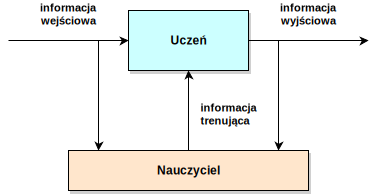
\includegraphics{graphics/01_podstawy_teoretyczne/supervised-learning.pdf}
	\caption{Uczenie maszynowe z nauczycielem \cite{CICHOSZ00}}
	\label{fig:supervised-learning}
\end{figure}

Uczeń otrzymuje od nauczyciela informację o tym jakiego komunikatu wyjściowego oczekuje w odpowiedzi na przykładowe informacje wejściowe, które mogą być dostarczone np. w formie wektorów. Na podstawie przykładów, system ma wyuczyć się reagowania na dane w odpowiedni, pożądany sposób.

%Uczenie nadzorowane przydaje się szczególnie do rozwiązania problemów związanych z klasyfikacją.

Inaczej jest w przypadku uczenia nienadzorowanego, gdzie nie występuje rola nauczyciela, a co za tym idzie, do systemu nie trafiają informacje instruktażowe. Wówczas dostępne są jedynie wektory wejściowe i na ich obserwacji uczeń ma nauczyć się odpowiednich odpowiedzi\cite{CICHOSZ00}.
%TODO napisac o zastosowaniu.. gdzies to bylo napisane
%TODO napisac co sie bardziej nadaje do rozwiazania problemy pracy mgr

Rzeczywiste dane wejściowe mogą się różnic od przykładowych danych służących do wytrenowania systemu. Umiejętność udzielania poprawnej odpowiedzi na komunikaty, które różnią się od przykładowych danych określamy jako generalizacja\cite{BISHOP06}.

\section{Rozpoznawanie obrazów}
%TODO ????
Lorem ipsum dolor sit amet, consectetur adipiscing elit. Suspendisse faucibus faucibus risus ut scelerisque. Curabitur in libero viverra, molestie ante in, scelerisque elit. Nam eu consequat metus. Vestibulum ante ipsum primis in faucibus orci luctus et ultrices posuere cubilia Curae; Nunc et vehicula est, et blandit turpis. Pellentesque nec pellentesque nisl. Nunc mattis porttitor urna, a varius sapien fringilla sed. Suspendisse sapien quam, mattis nec pretium ac, pharetra a ligula. Nunc sit amet porta arcu, id hendrerit dolor. Quisque placerat erat sit amet eros ornare, nec sollicitudin nunc pulvinar. Vivamus rutrum molestie magna, sed ornare neque consectetur non. Nam id quam metus.

In enim libero, imperdiet at dictum egestas, convallis sit amet eros. Vestibulum sed adipiscing purus, sed auctor metus. Morbi tempor, diam eu pretium sagittis, metus turpis hendrerit sem, a sollicitudin est massa ut odio. Sed blandit, felis sed semper mollis, diam nibh eleifend libero, pharetra eleifend ligula quam quis turpis. Donec vel fringilla arcu. Nullam suscipit congue elit, quis porta orci malesuada in. Quisque nisl arcu, tristique vel pretium ac, pulvinar et elit. Duis metus libero, iaculis et luctus nec, pulvinar feugiat leo. Curabitur vel tortor ut ligula dictum consequat ut sed ante. Aliquam nec odio ac ipsum facilisis aliquet quis in turpis. Cras tempor imperdiet erat, fringilla placerat urna tempus sollicitudin.

\section{Ekstrakcja cech}
%TODO problem ograniczania wielkosci wektora cech
%TODO podac przyklady z literatury jak robiono ekstrakcje poprzednio

Lorem ipsum dolor sit amet, consectetur adipiscing elit. Suspendisse faucibus faucibus risus ut scelerisque. Curabitur in libero viverra, molestie ante in, scelerisque elit. Nam eu consequat metus. Vestibulum ante ipsum primis in faucibus orci luctus et ultrices posuere cubilia Curae; Nunc et vehicula est, et blandit turpis. Pellentesque nec pellentesque nisl. Nunc mattis porttitor urna, a varius sapien fringilla sed. Suspendisse sapien quam, mattis nec pretium ac, pharetra a ligula. Nunc sit amet porta arcu, id hendrerit dolor. Quisque placerat erat sit amet eros ornare, nec sollicitudin nunc pulvinar. Vivamus rutrum molestie magna, sed ornare neque consectetur non. Nam id quam metus.

In enim libero, imperdiet at dictum egestas, convallis sit amet eros. Vestibulum sed adipiscing purus, sed auctor metus. Morbi tempor, diam eu pretium sagittis, metus turpis hendrerit sem, a sollicitudin est massa ut odio. Sed blandit, felis sed semper mollis, diam nibh eleifend libero, pharetra eleifend ligula quam quis turpis. Donec vel fringilla arcu. Nullam suscipit congue elit, quis porta orci malesuada in. Quisque nisl arcu, tristique vel pretium ac, pulvinar et elit. Duis metus libero, iaculis et luctus nec, pulvinar feugiat leo. Curabitur vel tortor ut ligula dictum consequat ut sed ante. Aliquam nec odio ac ipsum facilisis aliquet quis in turpis. Cras tempor imperdiet erat, fringilla placerat urna tempus sollicitudin.

\section{Klasyfikacja}
%TODO wymienic rozne rodzaje klasyfikatorow
%https://www.youtube.com/watch?v=qdDHp29QVdw
Lorem ipsum dolor sit amet, consectetur adipiscing elit. Suspendisse faucibus faucibus risus ut scelerisque. Curabitur in libero viverra, molestie ante in, scelerisque elit. Nam eu consequat metus. Vestibulum ante ipsum primis in faucibus orci luctus et ultrices posuere cubilia Curae; Nunc et vehicula est, et blandit turpis. Pellentesque nec pellentesque nisl. Nunc mattis porttitor urna, a varius sapien fringilla sed. Suspendisse sapien quam, mattis nec pretium ac, pharetra a ligula. Nunc sit amet porta arcu, id hendrerit dolor. Quisque placerat erat sit amet eros ornare, nec sollicitudin nunc pulvinar. Vivamus rutrum molestie magna, sed ornare neque consectetur non. Nam id quam metus.

In enim libero, imperdiet at dictum egestas, convallis sit amet eros. Vestibulum sed adipiscing purus, sed auctor metus. Morbi tempor, diam eu pretium sagittis, metus turpis hendrerit sem, a sollicitudin est massa ut odio. Sed blandit, felis sed semper mollis, diam nibh eleifend libero, pharetra eleifend ligula quam quis turpis. Donec vel fringilla arcu. Nullam suscipit congue elit, quis porta orci malesuada in. Quisque nisl arcu, tristique vel pretium ac, pulvinar et elit. Duis metus libero, iaculis et luctus nec, pulvinar feugiat leo. Curabitur vel tortor ut ligula dictum consequat ut sed ante. Aliquam nec odio ac ipsum facilisis aliquet quis in turpis. Cras tempor imperdiet erat, fringilla placerat urna tempus sollicitudin.

	\subsection{Klasyfikator według funkcji potencjału}
	Lorem ipsum dolor sit amet, consectetur adipiscing elit. Suspendisse faucibus faucibus risus ut scelerisque. Curabitur in libero viverra, molestie ante in, scelerisque elit. Nam eu consequat metus. Vestibulum ante ipsum primis in faucibus orci luctus et ultrices posuere cubilia Curae; Nunc et vehicula est, et blandit turpis. Pellentesque nec pellentesque nisl. Nunc mattis porttitor urna, a varius sapien fringilla sed. Suspendisse sapien quam, mattis nec pretium ac, pharetra a ligula. Nunc sit amet porta arcu, id hendrerit dolor. Quisque placerat erat sit amet eros ornare, nec sollicitudin nunc pulvinar. Vivamus rutrum molestie magna, sed ornare neque consectetur non. Nam id quam metus.

	In enim libero, imperdiet at dictum egestas, convallis sit amet eros. Vestibulum sed adipiscing purus, sed auctor metus. Morbi tempor, diam eu pretium sagittis, metus turpis hendrerit sem, a sollicitudin est massa ut odio. Sed blandit, felis sed semper mollis, diam nibh eleifend libero, pharetra eleifend ligula quam quis turpis. Donec vel fringilla arcu. Nullam suscipit congue elit, quis porta orci malesuada in. Quisque nisl arcu, tristique vel pretium ac, pulvinar et elit. Duis metus libero, iaculis et luctus nec, pulvinar feugiat leo. Curabitur vel tortor ut ligula dictum consequat ut sed ante. Aliquam nec odio ac ipsum facilisis aliquet quis in turpis. Cras tempor imperdiet erat, fringilla placerat urna tempus sollicitudin.
	
	\subsection{Klasyfikator statystyczny Bayesa}
	Lorem ipsum dolor sit amet, consectetur adipiscing elit. Suspendisse faucibus faucibus risus ut scelerisque. Curabitur in libero viverra, molestie ante in, scelerisque elit. Nam eu consequat metus. Vestibulum ante ipsum primis in faucibus orci luctus et ultrices posuere cubilia Curae; Nunc et vehicula est, et blandit turpis. Pellentesque nec pellentesque nisl. Nunc mattis porttitor urna, a varius sapien fringilla sed. Suspendisse sapien quam, mattis nec pretium ac, pharetra a ligula. Nunc sit amet porta arcu, id hendrerit dolor. Quisque placerat erat sit amet eros ornare, nec sollicitudin nunc pulvinar. Vivamus rutrum molestie magna, sed ornare neque consectetur non. Nam id quam metus.

	In enim libero, imperdiet at dictum egestas, convallis sit amet eros. Vestibulum sed adipiscing purus, sed auctor metus. Morbi tempor, diam eu pretium sagittis, metus turpis hendrerit sem, a sollicitudin est massa ut odio. Sed blandit, felis sed semper mollis, diam nibh eleifend libero, pharetra eleifend ligula quam quis turpis. Donec vel fringilla arcu. Nullam suscipit congue elit, quis porta orci malesuada in. Quisque nisl arcu, tristique vel pretium ac, pulvinar et elit. Duis metus libero, iaculis et luctus nec, pulvinar feugiat leo. Curabitur vel tortor ut ligula dictum consequat ut sed ante. Aliquam nec odio ac ipsum facilisis aliquet quis in turpis. Cras tempor imperdiet erat, fringilla placerat urna tempus sollicitudin.
	
	\subsection{Klasyfikator według minimalnej odległości}
	Lorem ipsum dolor sit amet, consectetur adipiscing elit. Suspendisse faucibus faucibus risus ut scelerisque. Curabitur in libero viverra, molestie ante in, scelerisque elit. Nam eu consequat metus. Vestibulum ante ipsum primis in faucibus orci luctus et ultrices posuere cubilia Curae; Nunc et vehicula est, et blandit turpis. Pellentesque nec pellentesque nisl. Nunc mattis porttitor urna, a varius sapien fringilla sed. Suspendisse sapien quam, mattis nec pretium ac, pharetra a ligula. Nunc sit amet porta arcu, id hendrerit dolor. Quisque placerat erat sit amet eros ornare, nec sollicitudin nunc pulvinar. Vivamus rutrum molestie magna, sed ornare neque consectetur non. Nam id quam metus.

	In enim libero, imperdiet at dictum egestas, convallis sit amet eros. Vestibulum sed adipiscing purus, sed auctor metus. Morbi tempor, diam eu pretium sagittis, metus turpis hendrerit sem, a sollicitudin est massa ut odio. Sed blandit, felis sed semper mollis, diam nibh eleifend libero, pharetra eleifend ligula quam quis turpis. Donec vel fringilla arcu. Nullam suscipit congue elit, quis porta orci malesuada in. Quisque nisl arcu, tristique vel pretium ac, pulvinar et elit. Duis metus libero, iaculis et luctus nec, pulvinar feugiat leo. Curabitur vel tortor ut ligula dictum consequat ut sed ante. Aliquam nec odio ac ipsum facilisis aliquet quis in turpis. Cras tempor imperdiet erat, fringilla placerat urna tempus sollicitudin.
	
	\subsection{Klasyfikator k Najbliższych Sąsiadów}
	Lorem ipsum dolor sit amet, consectetur adipiscing elit. Suspendisse faucibus faucibus risus ut scelerisque. Curabitur in libero viverra, molestie ante in, scelerisque elit. Nam eu consequat metus. Vestibulum ante ipsum primis in faucibus orci luctus et ultrices posuere cubilia Curae; Nunc et vehicula est, et blandit turpis. Pellentesque nec pellentesque nisl. Nunc mattis porttitor urna, a varius sapien fringilla sed. Suspendisse sapien quam, mattis nec pretium ac, pharetra a ligula. Nunc sit amet porta arcu, id hendrerit dolor. Quisque placerat erat sit amet eros ornare, nec sollicitudin nunc pulvinar. Vivamus rutrum molestie magna, sed ornare neque consectetur non. Nam id quam metus.

	In enim libero, imperdiet at dictum egestas, convallis sit amet eros. Vestibulum sed adipiscing purus, sed auctor metus. Morbi tempor, diam eu pretium sagittis, metus turpis hendrerit sem, a sollicitudin est massa ut odio. Sed blandit, felis sed semper mollis, diam nibh eleifend libero, pharetra eleifend ligula quam quis turpis. Donec vel fringilla arcu. Nullam suscipit congue elit, quis porta orci malesuada in. Quisque nisl arcu, tristique vel pretium ac, pulvinar et elit. Duis metus libero, iaculis et luctus nec, pulvinar feugiat leo. Curabitur vel tortor ut ligula dictum consequat ut sed ante. Aliquam nec odio ac ipsum facilisis aliquet quis in turpis. Cras tempor imperdiet erat, fringilla placerat urna tempus sollicitudin.

	\subsection{Maszyna wektorów wspierających (SVM)}
	Lorem ipsum dolor sit amet, consectetur adipiscing elit. Suspendisse faucibus faucibus risus ut scelerisque. Curabitur in libero viverra, molestie ante in, scelerisque elit. Nam eu consequat metus. Vestibulum ante ipsum primis in faucibus orci luctus et ultrices posuere cubilia Curae; Nunc et vehicula est, et blandit turpis. Pellentesque nec pellentesque nisl. Nunc mattis porttitor urna, a varius sapien fringilla sed. Suspendisse sapien quam, mattis nec pretium ac, pharetra a ligula. Nunc sit amet porta arcu, id hendrerit dolor. Quisque placerat erat sit amet eros ornare, nec sollicitudin nunc pulvinar. Vivamus rutrum molestie magna, sed ornare neque consectetur non. Nam id quam metus.

	In enim libero, imperdiet at dictum egestas, convallis sit amet eros. Vestibulum sed adipiscing purus, sed auctor metus. Morbi tempor, diam eu pretium sagittis, metus turpis hendrerit sem, a sollicitudin est massa ut odio. Sed blandit, felis sed semper mollis, diam nibh eleifend libero, pharetra eleifend ligula quam quis turpis. Donec vel fringilla arcu. Nullam suscipit congue elit, quis porta orci malesuada in. Quisque nisl arcu, tristique vel pretium ac, pulvinar et elit. Duis metus libero, iaculis et luctus nec, pulvinar feugiat leo. Curabitur vel tortor ut ligula dictum consequat ut sed ante. Aliquam nec odio ac ipsum facilisis aliquet quis in turpis. Cras tempor imperdiet erat, fringilla placerat urna tempus sollicitudin.
	
\section{Ocena klasyfikatorów}
%TODO jaka metode oceny bede uzywal w pracy?
Lorem ipsum dolor sit amet, consectetur adipiscing elit. Suspendisse faucibus faucibus risus ut scelerisque. Curabitur in libero viverra, molestie ante in, scelerisque elit. Nam eu consequat metus. Vestibulum ante ipsum primis in faucibus orci luctus et ultrices posuere cubilia Curae; Nunc et vehicula est, et blandit turpis. Pellentesque nec pellentesque nisl. Nunc mattis porttitor urna, a varius sapien fringilla sed. Suspendisse sapien quam, mattis nec pretium ac, pharetra a ligula. Nunc sit amet porta arcu, id hendrerit dolor. Quisque placerat erat sit amet eros ornare, nec sollicitudin nunc pulvinar. Vivamus rutrum molestie magna, sed ornare neque consectetur non. Nam id quam metus.

In enim libero, imperdiet at dictum egestas, convallis sit amet eros. Vestibulum sed adipiscing purus, sed auctor metus. Morbi tempor, diam eu pretium sagittis, metus turpis hendrerit sem, a sollicitudin est massa ut odio. Sed blandit, felis sed semper mollis, diam nibh eleifend libero, pharetra eleifend ligula quam quis turpis. Donec vel fringilla arcu. Nullam suscipit congue elit, quis porta orci malesuada in. Quisque nisl arcu, tristique vel pretium ac, pulvinar et elit. Duis metus libero, iaculis et luctus nec, pulvinar feugiat leo. Curabitur vel tortor ut ligula dictum consequat ut sed ante. Aliquam nec odio ac ipsum facilisis aliquet quis in turpis. Cras tempor imperdiet erat, fringilla placerat urna tempus sollicitudin.

%\section{Porównanie klasyfikatorów}
\include{02_porownanie}
\chapter{Implementacja}

Silnik kategoryzacyjny został zaimplementowany w języku C++, z użyciem środowiska Visual Studio w wersji 2010 Express, która jest czasowo ograniczona i bezpłatna do zastosowań niekomercyjnych.

\section{Język C++ i Visual Studio}

Język C++ jest językiem programowania ogólnego przeznaczenia. Jest językiem wieloparadygmatowym, czyli umożliwia stosowanie różnych paradygmatów programowania: proceduralnego, obiektowego i generycznego. Został zaprojektowany przez Bjarne Stroustrupa jako rozszerzenie języka C i użyty po raz pierwszy w 1979 roku. Charakteryzuje się obiektowymi mechanizmami abstrakcji danych oraz silną statyczną kontrolą typów.

Początkowo do realizacji zadania miał zostać wykorzystany język Python, ze względu na bogactwo bibliotek do uczenia maszynowego oraz przetwarzania obrazów. Warto wspomnieć szczególnie o dwóch bibliotekach: scikit-learn oraz scikit-image, które pozwalają na rozwiązanie wielu problemów związanych z klasyfikacją obrazów, klastrowaniem lub ekstrakcją cech. Zdecydowano o użyciu języka C++ z dwóch powodów:

\begin{compactitem}
	\item \emph{szybkość działania} -- kod jest kompilowany do kodu maszynowego, natomiast Python jest językiem interpretowanym i przez to czas potrzebny na osiągnięcie podobnych wyników jest większy
	\item \emph{silne typowanie} -- w przeciwieństwie do Pythona, język C++ jest silnie typowany, co w ocenie autora niniejszej pracy ma wpływ na zachowanie porządku w kodzie źródłowym
\end{compactitem}

Microsoft Visual Studio jest zintegrowanym środowiskiem programistycznym rozwijanym przez firmę Microsoft. 

\section{OpenCV}




\section{Architektura systemu}
...

\section{Opis API}
...
\chapter{Interpretacja wyników}

W celu określenia jakości działania silnika kategoryzacyjnego przeprowadzono kilka testów. Testy polegały na przeprowadzeniu kategoryzacji obrazów pochodzących ze zbioru Caltech-101.\cite{CALTECH101}

Caltech-101 jest zbiorem obrazów przygotowanych na Kalifornijskim Uniwersytecie Technicznym (w skrócie \emph{Caltech}) przez Fei-Fei Li, Marca Andreetto oraz Marca Aurelio Ranzato. Zawiera obrazy nieobciążone ograniczeniami licencyjnymi podzielone na 101 kategorii.

Testy zostały przeprowadzone dla 2, 4 oraz 8 kategorii, dla zbiorów zawierających 1, 5, 10, 15, 20, 30 oraz 40 obrazów na kategorię. Poniżej znajdują się wykresy trafności dla poszczególnych przypadków.

\begin{figure}[h]
	\centering
	\includegraphics[scale=0.8]{graphics/04_interpretacja_wynikow/result-sift-2.pdf}
	\caption{ Wykres trafności dla uczenia 2 kategorii (SIFT) }
	\label{fig:result-sift-2}
\end{figure}

\begin{figure}[h]
	\centering
	\includegraphics[scale=0.8]{graphics/04_interpretacja_wynikow/result-sift-4.pdf}
	\caption{ Wykres trafności dla uczenia 4 kategorii (SIFT) }
	\label{fig:result-sift-4}
\end{figure}

\begin{figure}[h]
	\centering
	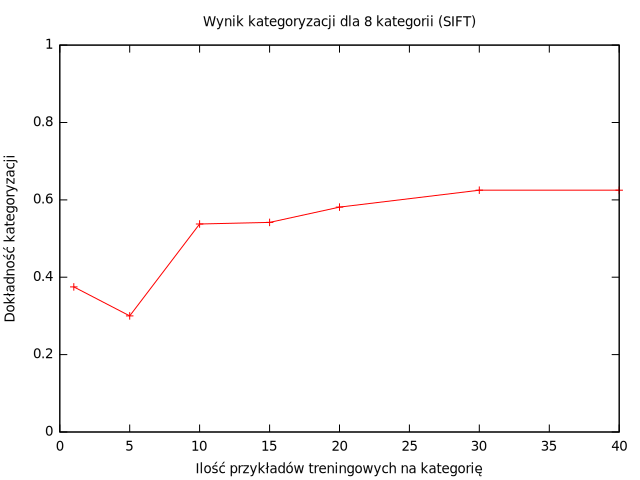
\includegraphics[scale=0.8]{graphics/04_interpretacja_wynikow/result-sift-8.pdf}
	\caption{ Wykres trafności dla uczenia 8 kategorii (SIFT) }
	\label{fig:result-sift-8}
\end{figure}

\begin{figure}[h]
	\centering
	\includegraphics[scale=0.8]{graphics/04_interpretacja_wynikow/result-surf-2.pdf}
	\caption{ Wykres trafności dla uczenia 2 kategorii (SURF) }
	\label{fig:result-sift-2}
\end{figure}

\begin{figure}[h]
	\centering
	\includegraphics[scale=0.8]{graphics/04_interpretacja_wynikow/result-surf-4.pdf}
	\caption{ Wykres trafności dla uczenia 4 kategorii (SURF) }
	\label{fig:result-sift-4}
\end{figure}

\begin{figure}[h]
	\centering
	\includegraphics[scale=0.8]{graphics/04_interpretacja_wynikow/result-surf-8.pdf}
	\caption{ Wykres trafności dla uczenia 8 kategorii (SURF) }
	\label{fig:result-sift-8}
\end{figure}
\chapter{Podsumowanie i zakończenie}

Różnorodność technik służących zarówno do ekstrakcji cech obrazów jak i klasyfikacji oraz dostępność dobrze udokumentowanych i zarazem darmowych bibliotek do przetwarzania obrazów pozwala na budowanie coraz skuteczniejszych narzędzi służących do kategoryzacji obrazów. Narzędzia te mogą być bardzo przydatne nie tylko do zapanowania nad zbiorami zdjęć, ale także mogą się przydać do budowy systemów zaawansowanego wyszukiwania grafiki na podstawie zapytań lub do szczegółowej analizy przeglądanych zdjęć w Internecie.

Narzędzie do kategoryzacji zdjęć zaproponowane w niniejszej pracy zostało oparte na metodzie \emph{Bag of Visual Words} i daje bardzo dobre wyniki dla 2 lub 4 kategorii. Wyniki przeprowadzonych testów pozwalają mieć nadzieję na to, że skuteczność metody dla przypadku większej ilości kategorii można poprawić poprzez dostrojenie parametrów maszyny wektorów nośnych oraz powiększenie zbiorów treningowych.

Zaproponowane API jest bardzo proste i umożliwia wykonanie podstawowych operacji na modelu oraz kategoryzację dowolnego obrazu. Silnik umożliwia też testowanie jakości kategoryzacji poprzez wskazanie trafności dla przykładowego scenariusza testowego. 

\section{Możliwe dalsze kierunki rozwoju}

W trakcie pisania niniejszej pracy magisterskiej pojawiło się kilka pomysłów, w jaki sposób można by było rozszerzyć zaproponowane rozwiązanie tak aby jego skuteczność była większa.

Zastosowanie dodatkowych deskryptorów, które są nieskorelowane z SIFT lub SURF mogłoby podnieść jakość kategoryzacji. Sensowne wydaje się zastosowanie technik GIST, niejako z definicji nie służące zastąpieniu deskryptorów SIFT/SURF ale mogące dodatkowo wesprzeć klasyfikator.

Dodatkowo wyznaczanie parametrów maszyny wektorów nośnych za pomocą prób i błędów można by zastąpić bardziej wyrafinowanymi sposobem opartym na walidacji krzyżowej.

\addcontentsline{toc}{chapter}{Bibliografia}
%%%%%%%%%%% Bibliografia %%%%%%%%%%%%%%%%%%%%%%%%%% 
\begin{thebibliography}{100} % 100 is a random guess of the total number of 
%references 

\bibitem{MARKETING12} Baier D., Daniel I., Frost S., \emph{Image data analysis and classification in marketing}, Advances in Data Analysis and Classification , Volume 6, Issue 4 , December 2012, Pages 253-276, ISSN 1862-5347

\bibitem{BAY08} Bay H., Ess A., Tuytelaars T., Van Gool L., \emph{SURF: Speeded Up Robust Features},  Computer Vision and Image Understanding (CVIU), Vol. 110, No. 3, 2008, Pages 346-359 

\bibitem{BISHOP06} Bishop C. M., \emph{Pattern Recognition and Machine Learning}, New York: Springer, 2006, ISBN 0-387-31073-8

\bibitem{CASEY} Casey C., \emph{Part Two: Like it or Not, Predictive Coding is Here and Judges Want you to Use it}, Hudson Legal Blog, 2012, http://us.hudson.com/legal/blog/postid/537/part-2 [dostep: 26.08.2014]

\bibitem{CHEN04} Chen Y., Wang J. Z., \emph{Image Categorization by Learning and Reasoning with Regions}, The Journal of Machine Learning Research, Volume 5, 2004, Pages 913-939 

\bibitem{CICHOSZ00} Cichosz P., \emph{Systemy uczące się}, Warszawa: Wydawnictwo Naukowo-Techniczne, 2000, ISBN 83-204-2544-1

\bibitem{DAI10} Dai D., Wu T., Zhu S-c., \emph{Discovering Scene Categories by Information Projection and Cluster Sampling}, CVPR 2010

\bibitem{GIST09} Douze M., Jégou H., Sandhawalia H., Amsaleg L, Schmid C.,\emph{Evaluation of GIST descriptors for web-scale image search}, Proceedings of the ACM International Conference on Image and Video Retrieval (CIVR '09). ACM, New York, 2009


\bibitem{GLAZER08} Glazer A., Sipper M., \emph{Evolving an Automatic Defect Classification Tool}, Applications of Evolutionary Computing, Heidelberg: Springer, 2008, Pages 194-203

\bibitem{GONZALES01} Gonzales R. C., Woods R. E., \emph{Digital Image Processing}, Boston MA, USA: Addison-Wesley Longman Publishing, 2001, ISBN 0201180758

\bibitem{GMM10} Górriz J. M., Segovia F., Ramírez J., Lassl A., Salas-Gonzalez D., \emph{GMM based SPECT image classification for the diagnosis of Alzheimer’s disease}, Applied Soft Computing, Volume 11, Issue 2, March 2011, Pages 2313-2325, ISSN 1568-4946

%TODO niecytowane
%\bibitem{HMS01} Hand D., Mannila H. Smyth P., \emph{Eksploracja danych}, Warszawa: Wydawnictwo Naukowo-Techniczne, 2005, ISBN 83-204-3053-4

\bibitem{HUANG11} Huang Y., Liu Q., Lv F., Gong Y., Dimitris N., \emph{Unsupervised Image Categorization by Hypergraph Partition}, Pattern Analysis and Machine Intelligence, IEEE Transactions, Volume 33, Issue 6, Pages 1266 - 1273

\bibitem{IMAGGA} Imagga APIs Documentation, http://docs.imagga.apiary.io/ [dostęp: 12.08.2014]

\bibitem{LINDENBERG90} Lindeberg T., \emph{Scale-space for discrete signals}, PAMI, 12(3), 1990, Pages 234–254

\bibitem{LZLM06} Liu Y., Zhang D., Lu G., Ma W-Y., \emph{A survey of content-based image retrieval with high-level semantics}, Pattern Recognition, Volume 40, Issue 1, January 2007, Pages 262-282, ISSN 0031-3203

\bibitem{MELE06} Mele K., Maver J., Sue D., \emph{Image Categorization Using Local Probabilistic Descriptors}, Pattern Recognition, 2006. ICPR 2006. 18th International Conference on  (Volume:2 ), Pages 336 - 340

\bibitem{MONTEJO13} Montejo L.D., Jia J., Kim H. K., Netz U. J., Blaschke S., Müller G. A., Hielscher A. H., \emph{Computer-aided diagnosis of rheumatoid arthritis with optical tomography, Part 2: image classification}, Journal of biomedical optics, Volume 18, Jul 2013, ISSN 1560-2281

\bibitem{NEUBECK06} Neubeck A., Van Gool L., \emph{Efficient non-maximum suppression}, ICPR, 2006

\bibitem{LEUNG00} Leung T., Malik J., \emph{Representing and Recognizing the Visual Appearance of Materials using Three-dimensional Textons},International Journal of Computer Vision, Volume 43 Issue 1, June 2001, Pages 29 - 44 

\bibitem{MOTODA98} Liu H., Motoda H., \emph{Feature Selection for Knowledge Discovery Data Mining}, Boston: Kluwer Academic Publishers, 1998

\bibitem{LOWE04} Lowe D. G., \emph{Distinctive Image Features from Scale-Invariant Keypoints}, International Journal of Computer Vision, Volume 60, Issue 2, November 2004, Pages 91 - 110 

\bibitem{SIFT99} Lowe D. G., \emph{Object Recognition from Local Scale-Invariant Features}, Proceedings of the International Conference on Computer Vision-Volume 2 - Volume 2 (ICCV '99), Vol. 2. IEEE Computer Society, 1999, Page 1150

\bibitem{LUO11} Luo H-L., Wei H., Hu F-X., \emph{Improvements in image categorization using codebook ensembles}, Image and Vision Computing, Volume 29, Issue 11, October 2011, Pages 759–773

\bibitem{OLIVA06} Oliva A., Torralba A., \emph{Building the gist of a scene: the role of global image features in recognition}, Progress in Brain Research, Vol. 155, 2006, Pages 23-36

\bibitem{OLIVA00} Oliva A., Torralba A., \emph{Modeling the Shape of the Scene: A Holistic Representation of the Spatial Envelope}, International Journal of Computer Vision, May 2001, Volume 42, Issue 3, pp 145-175

\bibitem{PIXIT} PiXiT, http://www.montefiore.ulg.ac.be/~maree/pixit.html [dostęp: 12.08.2014]

\bibitem{SCHWEIGER09} Schweiger F., Zeisl B., Georgel P et al.: Maximum Detector Response Markers for SIFT and SURF, VMV, 
2009

\bibitem{SCHYNS94} Schyns P.G., Oliva A., \emph{From blobs to boundary edges: evidence for time- and spatial-scale-dependent scene} recognition, 1994, Psychol. Sci., 5, Pages 195–200

\bibitem{Google2010} Smith N., \emph{Ooh! Ahh! Google Images presents a nicer way to surf the visual web}, Google Official Blog, 2010, http://googleblog.blogspot.com/2010/07/ooh-ahh-google-images-presents-nicer.html [dostęp: 05.08.2014]

\bibitem{STRUMIL} Strumillo P., \emph{Przetwarzanie obrazów, wykłady}, http://www.eletel.p.lodz.pl/pstrumil/ [dostęp: 6.09.2014]

\bibitem{SUVDAA2012} Suvdaa B., Ahn J., Ko J., \emph{Steel Surface Defects Detection and Classification Using SIFT and Voting Strategy}, International Journal of Software Engineering and Its Applications, Volume 6, No. 2, Apri 2012, Pages 161-166

\bibitem{Tad91} Tadeusiewicz R., Flasiński M., \emph{Rozpoznawanie obrazów}, Warszawa: Państwowe Wydawnictwo Naukowe, 1991, ISBN 83-01-10558-5

\bibitem{WARWICK10} Wernick M.N., Yongyi Y., Brankov J.G., Yourganov G., Strother S.C., \emph{Machine Learning in Medical Imaging}, Signal Processing Magazine, IEEE, Volume 27,  Issue 4, July 2010, Pages 25-38

\bibitem{VALPOLA} Valpola H., \emph{Bayesian Ensemble Learning for Nonlinear Factor Analysis}, Acta Polytechnica Scandinavica, Mathematics and Computing Series No. 108, Espoo 2000, 54 pp.

\bibitem{VISWANATHAN08}  Viswanathan M., Siagian C., Itti L., \emph{Comparisons of Gist Models in Rapid Scene Categorization Tasks}, 2008

\bibitem{Vitaladevuni13} Vitaladevuni S.N., Natarajan P. ; Shuang W., Xiaodan Z., Prasad R. , Natarajan P., \emph{Scene image categorization and video event detection using Naive Bayes Nearest Neighbor}, Applications of Computer Vision (WACV), 2013 IEEE Workshop on, 2013, Pages 140 - 147
 
\end{thebibliography} 
%%%%%%%%%%%%% end %%%%%%%%%%%%%%%%%%%%%%%%%%%%%%% 
\end{document}
